%%%%%%%%%%%%%%%%%%%%%%%%%%%%%%%%%%%%%%%%
%%%%%  Chapitre Installation
%%%%%%%%%%%%%%%%%%%%%%%%%%%%%%%%%%%%%%%%

\chapter{Installation}  \index[con]{installation}

Les installations présentées ici sont sous Windows. Pour une installation Mac, il convient de consulter le document de Fabien \textsc{Conus} et de Franck \textsc{Pastor}\cite{conu}.

L'installation de \LaTeX\ est très fortement marquée par l'aspect modulaire de ce programme : beaucoup de fichiers sont créés et dépendent les uns des autres. Par ailleurs, \LaTeX\ crée par défaut des documents affichables mais non imprimables. L'installation de certains programmes complémentaires permet de convertir ces documents dans des formats imprimables. 


\section{Une installation compacte : USB\TeX}

L'installation retenue pour le cours est USB\TeX\ du fait de sa simplicité d'utilisation. Il s'agit d'un regroupement de plusieurs programmes de taille réduite : la distribution (voir ci-dessous) MiK\TeX, les programmes \programme{Ghostscript}, \programme{GSview} et l'éditeur \programme{Texmaker}.

\subsection{Installation}

Le fichier exécutable d'un peu plus de 150~Mo est téléchargeable par le biais du site de Framasoft\footnote{\liensimple{http://www.framasoft.net/article4641.html}. S'y trouve également le mode d'emploi résumé ci-dessus.}. L'exécution de ce fichier le fait se décompresser dans le répertoire demandé par la fenêtre qui s'affiche alors. Ceci fait, il faut se placer dans le répertoire nouvellement créé par l'installation\footnote{Ce répertoire est nommé \vue{USBTeX-} suivi du numéro de version d'USB\TeX.} et cliquer sur le raccourci nommé  \vue{Texmaker} pour pouvoir utiliser l'éditeur \programme{Texmaker}.  

\subsection{Maintenance}

\subsubsection{Cas usuel}

L'installation initiale faite ci-dessus inclut un nombre restreint de paquet. Si, lors d'une compilation, un paquet semble manquant pour l'installation, \programme{Texmaker} vous propose de l'installer directement par téléchargement en ligne (en passant par le logiciel de maintenance de MiK\TeX). Ceci évite de se poser des questions concernant les paquets, leur installation et leur maintenance. 

\subsubsection{Cas moins usuel}

L'installation de paquet peut aussi se faire de façon plus manuelle en allant directement installer les paquets souhaités. Pour le faire, il faut lancer le raccourci \vue{MiKTeX} présent dans le répertoire créé par l'installation. 

Ceci fait apparaître une nouvelle icône dans la barre des tâches. En cliquant avec le bouton droit dessus et en sélectionnant \vue{MiKTeX Package Manager} se lance alors le gestionnaire de paquet. Il peut mettre un certain temps avant de réagir car il compare les paquets présents et les paquets disponibles. Une fois la liste des paquets affichée, il suffit de sélectionner ici n'importe quel paquet et de cliquer sur l'icône \vue{+} pour l'installer.

\subsubsection{Cas improbable mais vrai}

Il peut arriver que des problèmes de configuration de connexion empêche d'utiliser ce système directement. Si la connexion internet est fonctionnelle, il est possible de contourner cette difficulté en récupérant soi-même les fichiers que va chercher le gestionnaire de paquets sur des dépôts (\emph{repository} en anglais) et en les stockant dans un répertoire dédié sur son ordinateur. 

Une fois connue l'adresse d'un dépôt\footnote{Par exemple \liensimple{ftp://ftp.dante.de/pub/tex/systems/win32/miktex/tm/packages/}. Une liste de dépôts est disponible à l'adresse \liensimple{http://miktex.org/pkg/repositories}.}, il faut alors y récupérer et placer dans un unique répertoire de son ordinateur les éléments suivants :
\begin{itemize}
\item les fichiers dont le nom commence par \vue{miktex-zzdb} ;
\item les fichiers des paquets qui vous intéressent.
\end{itemize}

Le premier ensemble de fichiers sert à indiquer la liste des paquets du dépôt au gestionnaire de paquet. En l'absence de ces fichiers, le gestionnaire de dépôt refusera de prendre en compte votre répertoire.

Dans le gestionnaire de paquet MiK\TeX, il faut alors aller dans le menu \vue{Repository} puis \vue{Change Package Repository}, sélectionner alors la ligne \vue{... from a directory} puis \vue{Suivant}, sélectionner le répertoire où sont vos paquets et cliquer enfin sur \vue{Terminer}.

\subsection{La vérification orthographique}

L'installation sur clé présente une coquille pour ce qui est du correcteur orthographique. Il faut modifier le chemin présent dans le menu \vue{Options}, \vue{Configurer Texmaker} puis \vue{Editeur}. Le chemin de la ligne \vue{Dictionnaire} est à modifier par le biais de la petite icône à côté de la zone de saisie du chemin, en cherchant le répertoire où est installé USBTeX (\vue{USBTeX-1.7}) puis en allant dans le sous-répertoire \vue{programs} puis \vue{Texmaker} et sélectionner alors le fichier \vue{fr\_FR.dic}. 

\section{Une installation complète}

Le côté pratique d'USB\TeX\ cache les liens entre les différents programmes. Est donc décrite ici une installation complète\footnote{Parmi d'autres possibles telle \liensimple{http://www.xm1math.net/doculatex/install_miktex.html}.} sous Windows. Celle-ci demande de récupérer trois ensembles :
\begin{itemize}
\item une \terme{distribution} de \LaTeX, autrement dit \LaTeX\ et de nombreux programmes et fichiers satellites (paquets, documentations, formats...) ;
\item \programme{Ghostscript} et \programme{GSview} qui gèrent le postscript et les fichiers \dextension{ps} et \dextension{eps} ;
\item un éditeur \LaTeX, point vu en section \ref{éditeurs}.
\end{itemize}

% install-tl-windows.bat
\subsection{\LaTeX}

La distribution retenue ici de \LaTeX\ est la \TeX Live 2014, soumise à la licence GNU\footnote{Licence qui gère le logiciel libre.}. La dernière distribution de la \TeX live est disponible sur \liensimple{http://www.tug.org/texlive/}. Plusieurs modes d'installation sont possibles :
\begin{itemize}
\item en téléchargeant un fichier d'installation qui récupère les différents fichiers nécessaires sur le web. Il se trouve sur le site en suivant le lien \vue{Download} puis le lien \vue{install-tl.zip}.\index[con]{texlive@\TeX Live} Une fois ce fichier décompressé, il faut exécuter le programme \vue{install-tl.bat}, qui affiche la fenêtre de la figure \ref{figtexlive} ;
\item en téléchargeant le DVD d'installation présent sur le site\footnote{Actuellement, l'adresse donnée est la suivante : \liensimple{http://mirrors.ircam.fr/pub/CTAN/systems/texlive/Images/texlive2014-20140525.iso}.}. Ce fichier doit alors être gravé ou monté sur un lecteur virtuel. Une fois lancé, il faut lancer le fichier \vue{install-tl-windows.bat} qui affiche le même menu qu'à la méthode précedente.
\end{itemize}

\begin{figure}[H]
\centering 
\resizebox{10cm}{!}{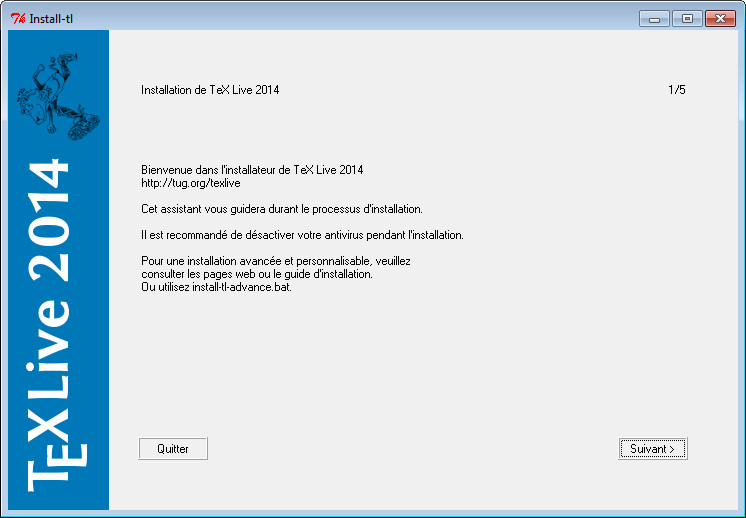
\includegraphics{images/texlive2014.jpg}}
\caption{Page d'accueil de \TeX Live 2014}\label{figtexlive}
\end{figure}

Les différents choix usuels de configuration sont récapitulés dans le tableau suivant à raison d'une ligne par fenêtre d'installation.

\begin{table}[H]
\centering
\begin{tablecouleur}
\begin{tabular}{cl}
\rowcolor{bleu20}
\color{white}\bf Fenêtre &  \multicolumn{1}{c}{\color{white}\bf Action}	\\ 
1/5 & Suivant 															\\ 
2/5 & Répertoire \vue{C:\ba TeXLive\ba 2014}. Suivant 	\\
3/5 & Suivant 															\\ 
4/5 & Installer 														\\ 
5/5 & Attendre et quitter 												\\
\end{tabular}
\end{tablecouleur}
\caption{\'{E}tapes d'installation de la \TeX live 2014}
\end{table}

Cette partie est assez longue, surtout si c'est la méthode du fichier d'installation qui est retenue : les différents fichiers constitutifs de l'installation seront tous téléchargés. Dans la mesure où il y a beaucoup de fichiers de taille variable, la durée de téléchargement est elle-même délicate à mesurer. Par expérience, il faut compter deux bonnes heures. 

Avec la méthode par DVD, le temps d'installation passe environ à une demi-heure.

\subsection{\programme{Ghostscript} et \programme{GSview}}
\subsubsection{\programme{Ghostscript}} 

\programme{Ghostscript} permet de travailler avec des fichiers postscript ou \dextension{ps} ainsi que les images au format \dextension{eps}. Avec le programme \programme{ps2pdf} compris dans les programmes fournis avec \programme{Ghostscript}, il devient possible de convertir un fichier \dextension{ps} en \dextension{pdf}. 

Une fois le programme dans sa version libre non commerciale (nommée GPL ou \emph{General Public License}) téléchargé\footnote{Il se trouve à l'adresse \liensimple{http://www.ghostscript.com/download/gsdnld.html}.}, il convient de suivre la suite d'instructions présentée ci-après.

\begin{table}[H]
\centering
\begin{tablecouleur}
\begin{tabular}{cl}
\rowcolor{bleu20}
\color{white}\bf Fenêtre 	& \multicolumn{1}{c}{\color{white}\bf Action}		\\ 
Welcome						& Next    											\\ 
License agreement			& I agree 											\\
Choose install				& Répertoire \vue{C:\ba Texlive\ba gs}. Install		\\
Completing					& Finish 											\\
\end{tabular}
\end{tablecouleur}
\caption{\'{E}tapes d'installation de \programme{Ghostscript}}
\end{table}


\subsubsection{\programme{GSview}}
  
\programme{GSview} est un outil graphique qui facilite grandement l'utilisation de \programme{Ghostscript}. Grâce à lui, la visualisation d'un document \dextension{ps} est simplifiée. 

La version de \programme{GSview} à télécharger\footnote{À l'adresse \liensimple{http://pages.cs.wisc.edu/~ghost/gsview/index.htm}, en retenant par rapport à la remarque ci-dessus la version \vue{GSview release v5.0}.} doit être compatible avec la version de \programme{Ghostscript}. Une fois lancé l'exécutable, les étapes de configuration sont indiquées ci-après.

\begin{table}[H]
\centering
\begin{tablecouleur}
\begin{tabular}{cl}
\rowcolor{bleu20}
\color{white}\bf Fenêtre 	& \multicolumn{1}{c}{\color{white}\bf Action}			\\ 
Winzip Self-Extractor	 	& Setup     											\\
Select Language 			& Francais 												\\
This wizard will		 	& Next		   											\\
Copyright					& Next   												\\
GSview can create	 		& Next	   												\\
Select a directory			& Répertoire \vue{C:\ba Texlive\ba Ghostgum}. Next		\\
The directory you			& Next		   											\\
GSview setup will			& Finish	  											\\
Installation successful		& Exit 													\\
\end{tabular}
\end{tablecouleur}
\caption{\'{E}tapes d'installation de \programme{GSview}}
\end{table}

Point important, il faut lancer une première fois \programme{GSview} pour le configurer. Sans cela, il indiquera systématiquement une erreur à l'ouverture d'un fichier \dextension{ps}. Une fois lancé, il faut aller dans le menu \vue{Options} puis \vue{Easy Configure} et sélectionner le numéro de version de \programme{Ghostscript}\footnote{Ce dernier est dans le nom du fichier d'installation de \programme{Ghostscript}.}. \programme{GSview} peut alors être fermé.


\subsection{Configuration de Windows}

Les différentes versions de Windows réagissent diversement à l'installation de \LaTeX. La plupart des versions\footnote{Windows 7 semble faire exception.} ne feront pas fonctionner \programme{ps2pdf}, mystérieusement introuvable. Il faut comprendre par là que lorsque Windows cherche un programme, il parcourt une liste de répertoires bien spécifiques et, dans notre cas, nos répertoires contenant \LaTeX\ ou \programme{Ghostscript} n'en font pas partie.

Pour corriger ce point, il faut modifier la variable \vue{Path} des variables d'environnement. Dans le panneau de configuration, double-cliquer sur \vue{Système}\footnote{Dans le cas de Windows XP, il faut d'abord cliquer sur l'icône \vue{Performance et maintenance}. Pour Windows Vista, il faut demander l'affichage \og classique \fg, l'icône \vue{Système} apparaissant alors.}. Sélectionner alors l'onglet avancé et cliquer alors sur \vue{Variables d'environnement}. 

\begin{figure}[H]
\centering
\resizebox{10cm}{!}{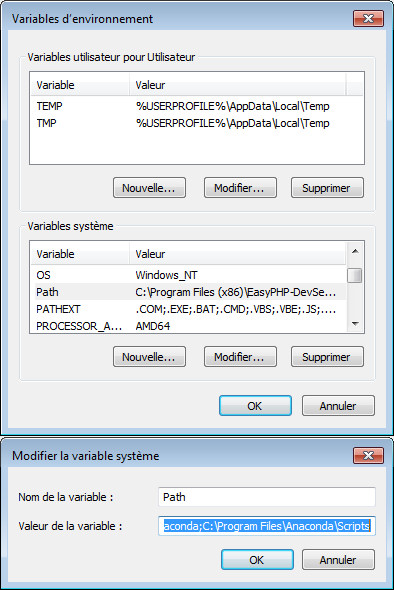
\includegraphics{images/variables.jpg}}
\caption{Exemple d'entrée des chemins sous Windows XP}
\end{figure}

Là, il faut sélectionner la ligne \vue{Path} et cliquer sur \vue{Modifier}. On ajoute alors\footnote{... sans effacer les chemin déjà présents !} les chemins vers nos programmes, autrement dit la ligne suivante\footnote{Les points-virgules servent ici de séparateurs entre les différents chemins.} :
\begin{center}
\vue{\footnotesize\texttt{;C:\ba Texlive\ba bin\ba win32\ba;C:\ba Texlive\ba gs\ba gs9.06\ba bin\ba;C:\ba Texlive\ba gs\ba gs9.06\ba lib\ba}}
\end{center}


\section{Des éditeurs} \label{éditeurs}

Une fois les différents programmes fondamentaux installés, il faut installer un programme permettant d'éditer de façon simple les documents \dextension{tex} et de lancer aisément des compilations ou des conversions de document. Ce document en présente deux. 

Dans tous les cas, un point d'attention est porté sur la configuration car il faut systématiquement indiquer à ces programmes où se trouvent les différents programmes que nous avons installé précédemment.


\subsection{\programme{Texmaker}}

Programme libre sous licence GNU, \programme{Texmaker}\footnote{Il est téléchargeable à l'adresse \liensimple{http://www.xm1math.net/texmaker/index_fr.html}.} est un des logiciels de référence pour l'édition de documents \dextension{tex}. L'installation se limite tout au mieux à indiquer le répertoire où sera installé le programme. Le paramétrage des programmes s'obtient par le menu \vue{Options}, \vue{Configurer Texmaker}. L'image ci-dessous\footnote{Cette présentation dépend de la version de \programme{Texmaker} mais contient le même type d'information.} donne la configuration attendue par défaut.

\begin{figure}[H]
\centering
\resizebox{14cm}{!}{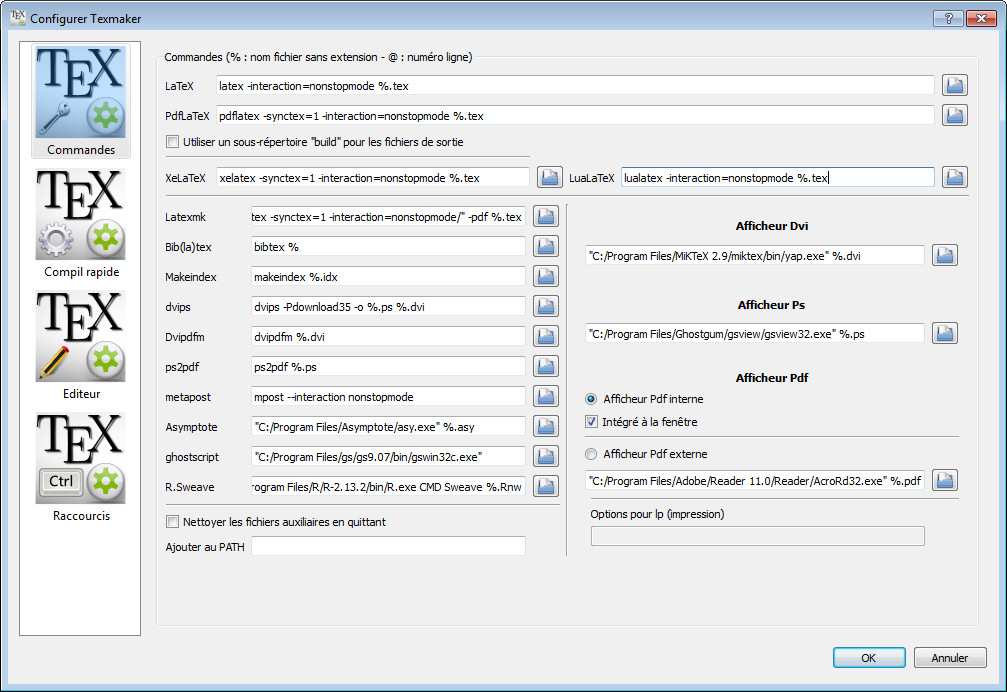
\includegraphics{images/texmaker441.jpg}}
\caption{Paramétrage de \programme{Texmaker}}
\end{figure}

\programme{Texmaker} gère l'encodage UTF8. Il s'agit d'une norme de saisie des caractères qui se répand de plus en plus car elle permet de gérer de très nombreuses langues. Si vous utilisez UTF8, il faut modifier le préambule de notre document, en remplaçant \macron{latin1} par \macron{utf8}. 

\begin{codesimple}{Code pour l'UTF8}{codeutf}
\usepackage[utf8]{inputenc}
\end{codesimple}

Selon la version de \programme{Texmaker}, la gestion de l'UTF8 n'est pas systématique. Il faut parfois modifier directement l'encodage utilisé par défaut. Ceci se fait dans le menu \vue{Options}, \vue{Configurer Texmaker}, \vue{Editeur} en paramétrant dans l'encodage \vue{UTF-8}.

\subsection{\programme{TeXnicCenter}}

\programme{TeXnicCenter}\footnote{Téléchargeable à l'adresse \liensimple{http://www.texniccenter.org/}.} offre une large panoplie de fonctionnalités, à l'image de \programme{Texmaker}. L'installation propose un peu plus de choix que dans \programme{Texmaker} et demande également la localisation des fichiers de la distribution\footnote{Il faut indiquer le répertoire \vue{C:\ba Texlive\ba 2014\ba bin\ba win32} si vous avez suivi le paramétrage proposé dans ce document.}. Les options proposées restent lisibles et rendent cette phase peu difficile. 

L'installation vous demandant de lui indiquer où est la distribution, il n'y a pas ou peu d'actions à faire pour configurer \programme{TeXnicCenter}. \`{A} titre d'information,  cette opération se fait dans le menu \vue{Build} puis \vue{Define Output Profiles}. 

\begin{figure}[H]
\centering
\resizebox{12cm}{!}{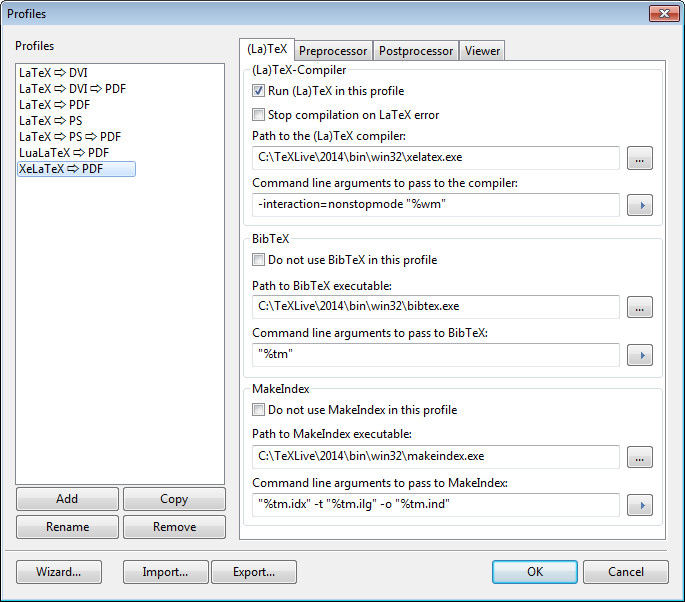
\includegraphics{images/texniccenter.jpg}}
\caption{Paramétrage de \programme{TeXnicCenter}}
\end{figure}